\section{Дополнительные примеры чувствительности нейтринной томографии к профилю плотности Земли}
\label{sec:appTomography}

В дополнение к сценарию, рассмотренному в основном тексте, проанализируем ещё два варианта распределения плотности, отличающихся от стандартной модели PREM.  
Для каждого случая вычислены значения статистики $\Delta\chi^2$, характеризующие степень различия с моделью PREM при предположении нейтринного телескопа объёмом $1~\text{км}^3$ и времени наблюдения один год.

\subsection{Усреднённое ядро}

В качестве альтернативной гипотезы $H_1$ рассмотрим модель, в которой плотность вещества принимается постоянной и равной $\rho = 11.87~\text{г/см}^3$ во всей области внутреннего и внешнего ядра, тогда как мантия описывается стандартной моделью PREM.  
Для пары гипотез ($H_0$, $H_1$) получено $\Delta\chi^2 = 0.114$, что соответствует статистической значимости $0.34\sigma$.  
Если увеличить время наблюдения до 25 лет либо использовать нейтринный телескоп существенно большего объёма (например, $30~\text{км}^3$), ожидаемая значимость возрастает до $\sim 2\sigma$.

\begin{figure}[!h]
    \centering
    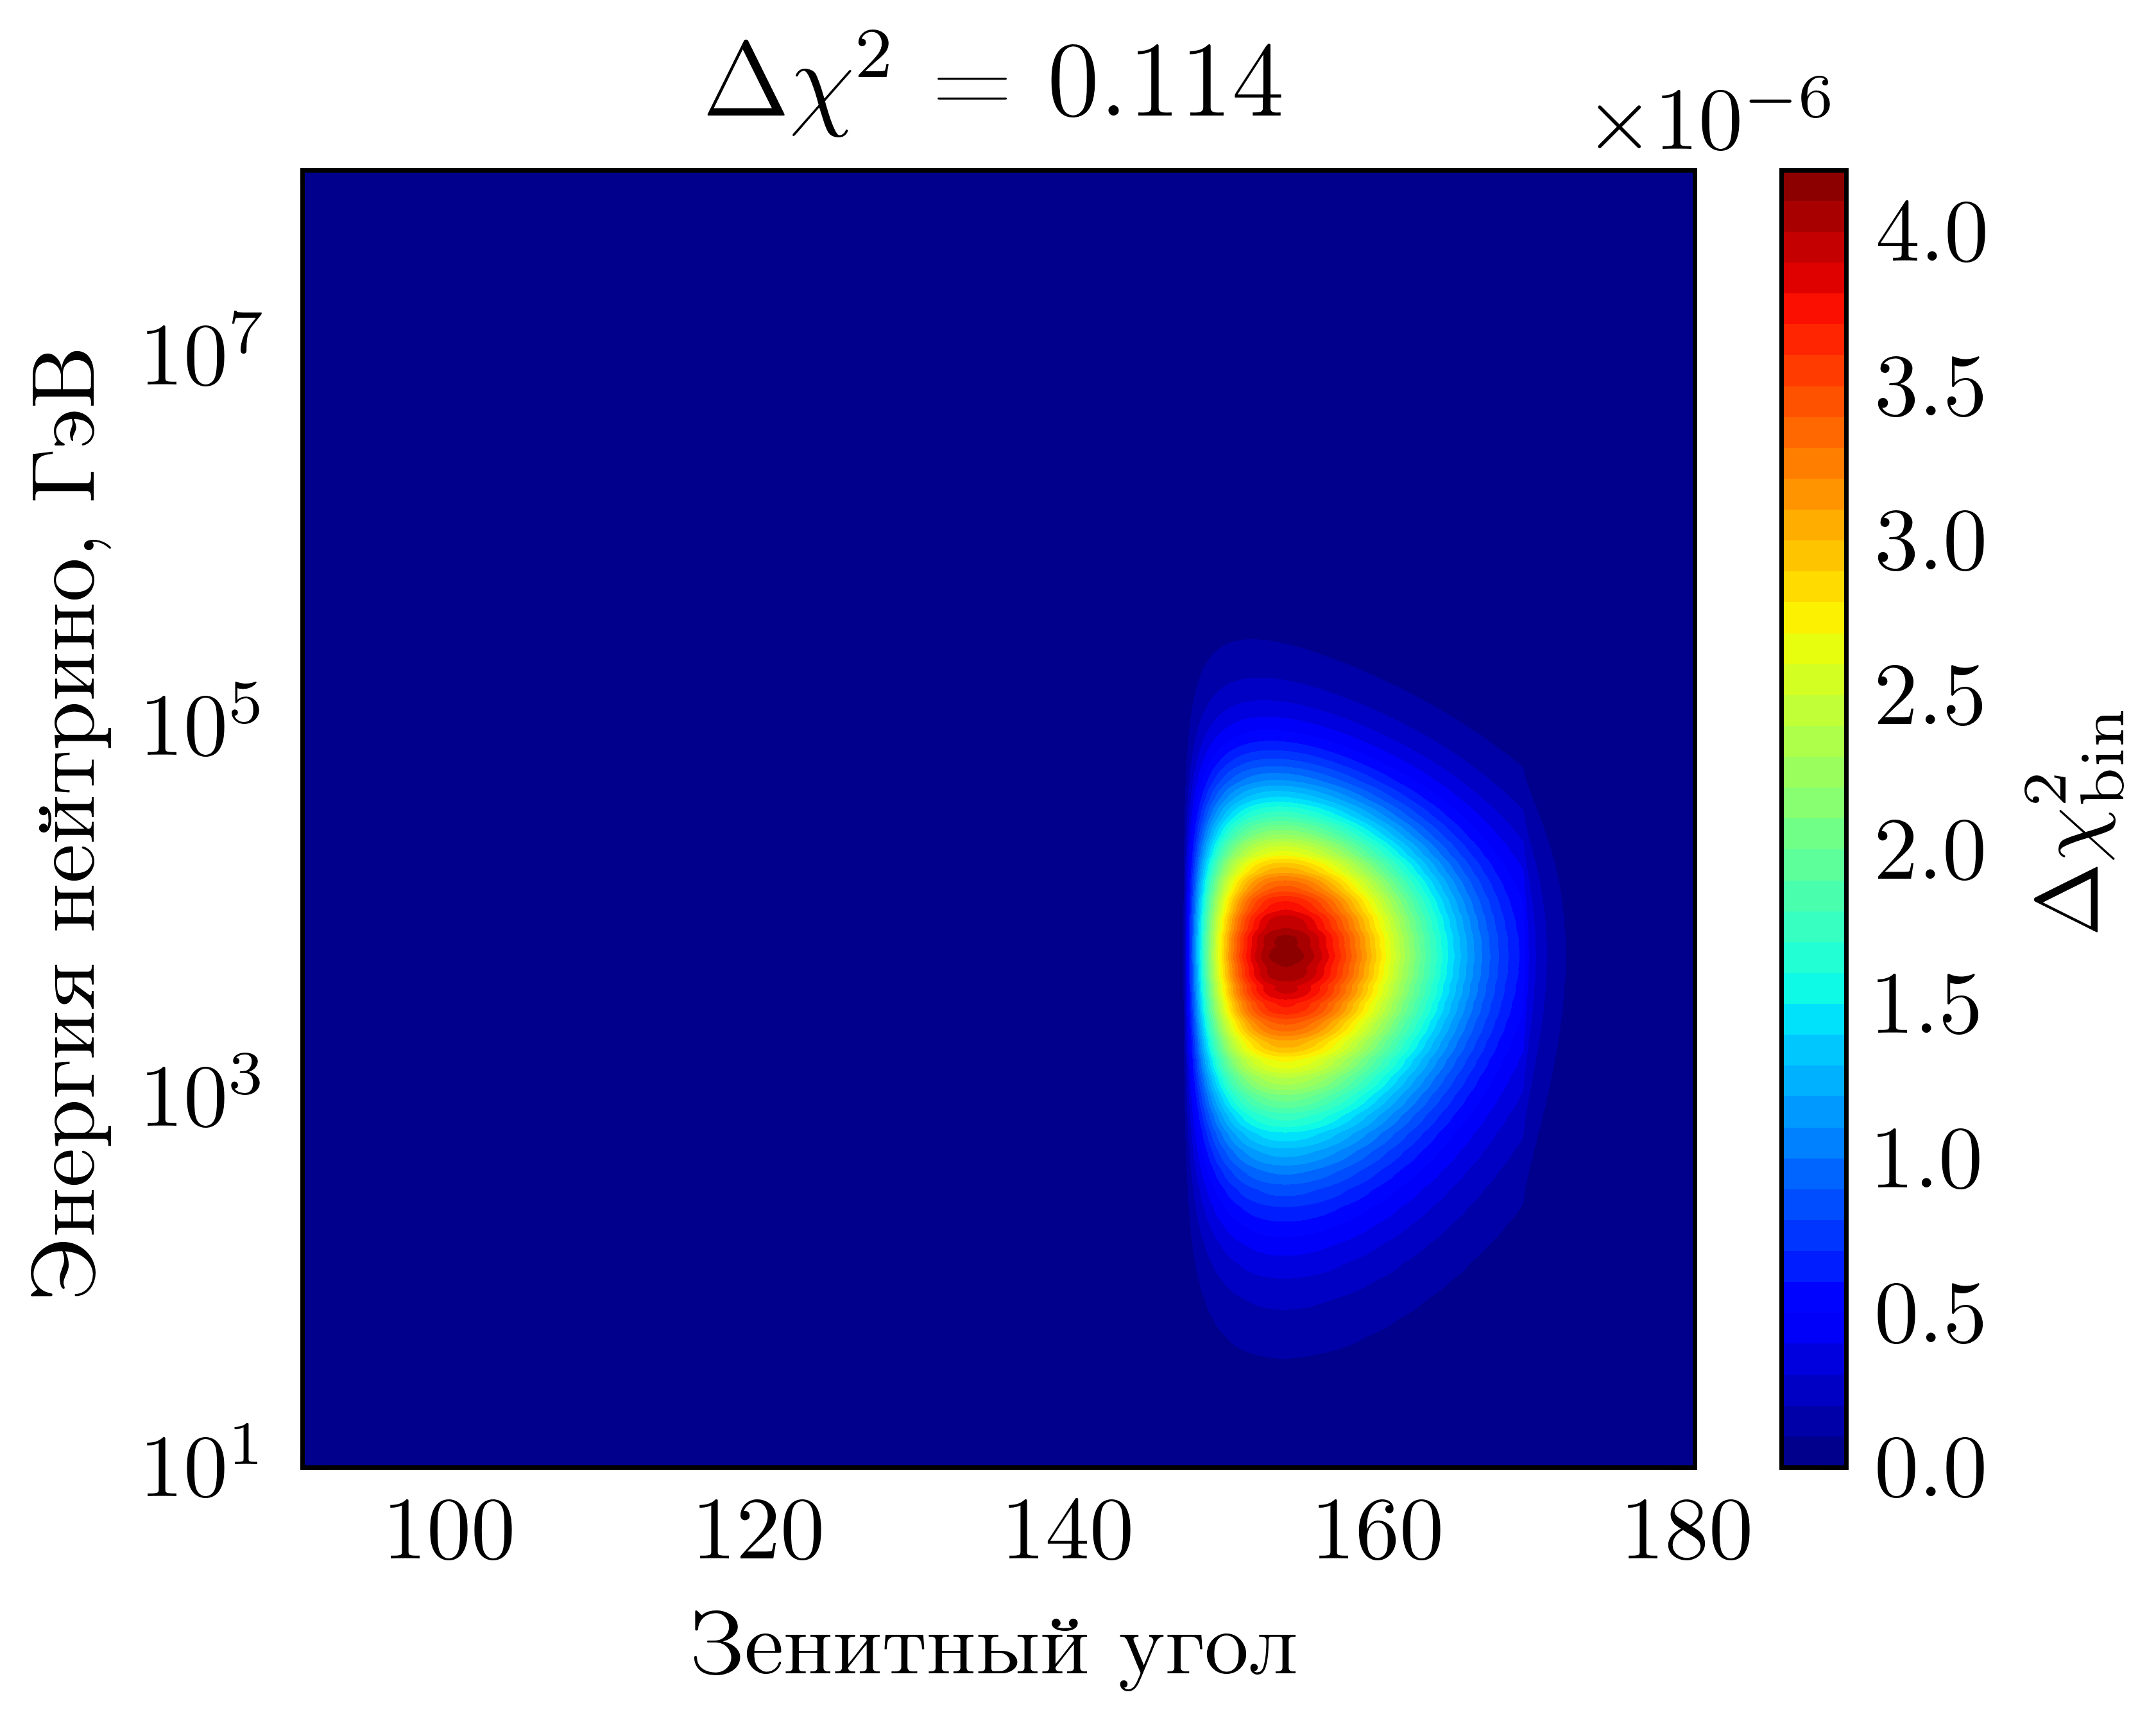
\includegraphics[width=\linewidth]{images/NuProp/chi2_rzf_2dxsCT10nlo_PREM_vs_PREM_av_ext_ker.png}
    \caption{Распределение статистики $\Delta\chi^2$, полученное при сравнении числа нейтринных событий для гипотез $H_0$ (модель PREM) и $H_1$ (усреднённое ядро).}
    \label{NuTom2}
\end{figure}

\subsection{Линейное ядро}

В следующем сценарии в качестве альтернативной гипотезы используется модель, в которой плотность в области внутреннего и внешнего ядра аппроксимируется линейной функцией радиуса.  
Вне ядра распределение плотности совпадает с моделью PREM.  
Для этой пары гипотез ($H_0$, $H_1$) получено $\Delta\chi^2 = 0.601$, что соответствует статистической значимости $0.76\sigma$.  
При увеличении времени наблюдения до десяти лет ожидаемая значимость достигает $\sim 2.5\sigma$.

\begin{figure}[!h]
    \centering
    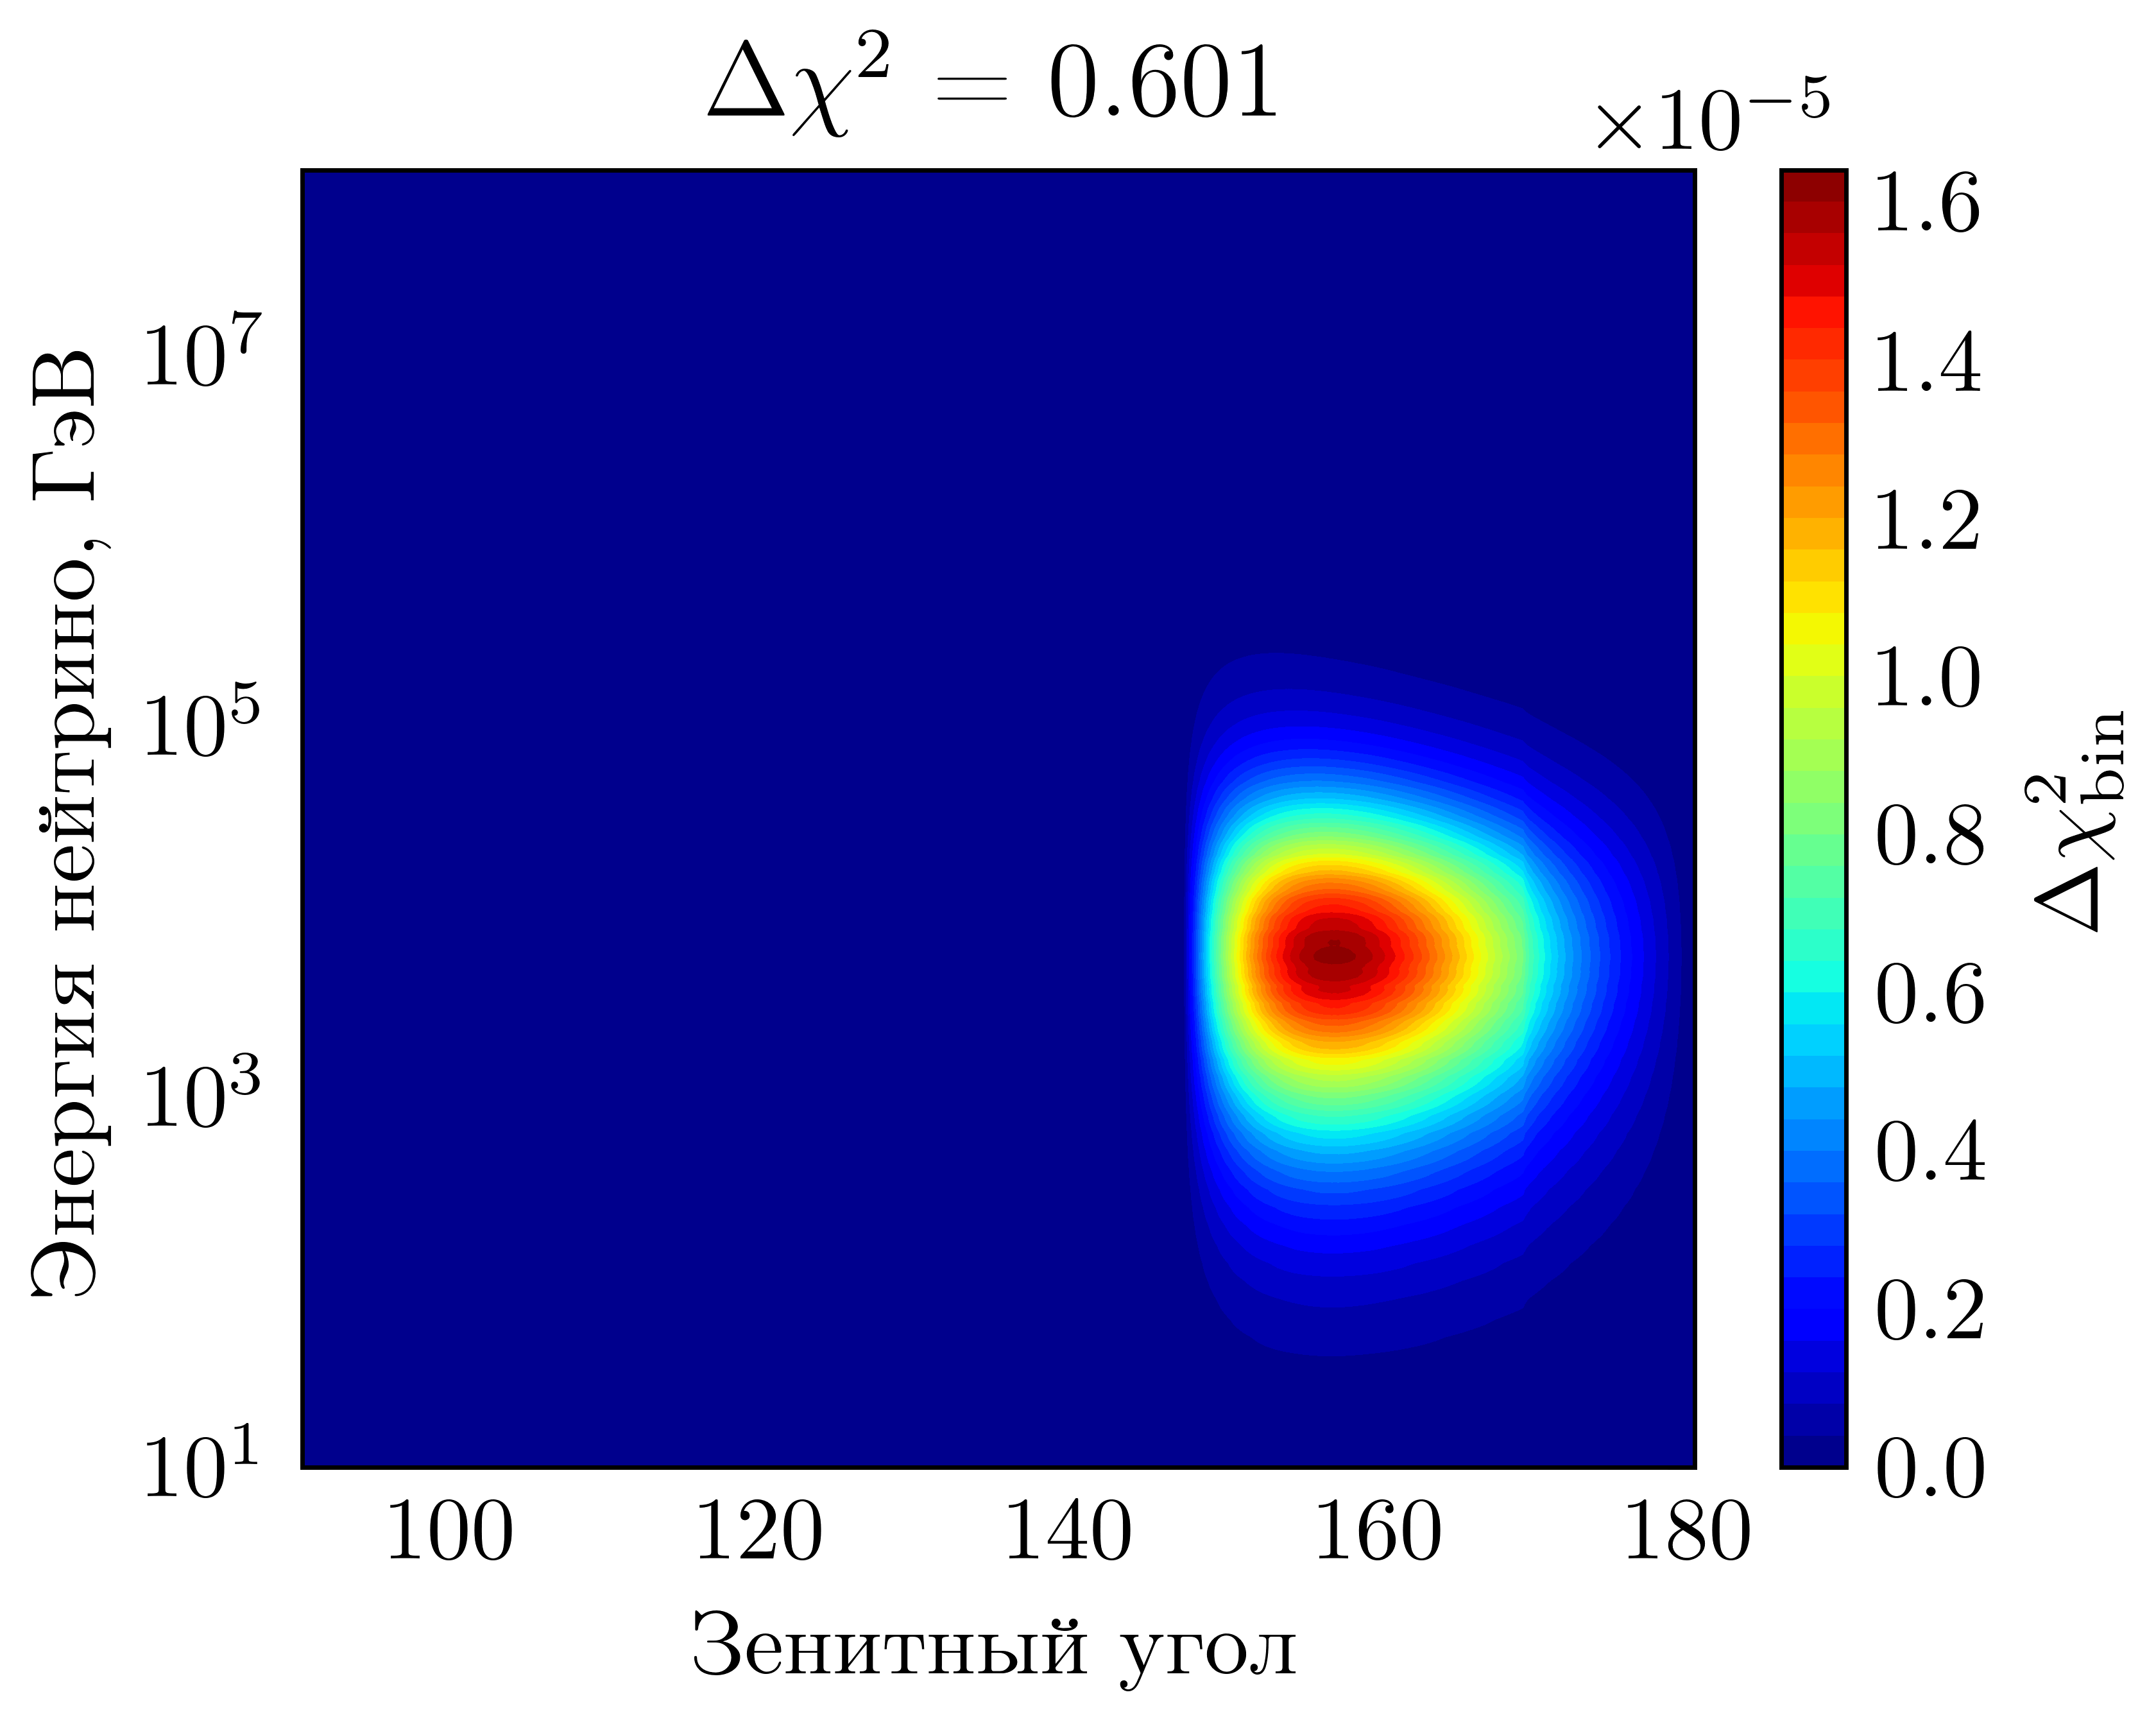
\includegraphics[width=\linewidth]{images/NuProp/chi2_rzf_2dxsCT10nlo_PREM_vs_PREM_lin_ker.png}
    \caption{Распределение статистики $\Delta\chi^2$ для гипотез $H_0$ (модель PREM) и $H_1$ (линейное ядро).}
    \label{NuTom3}
\end{figure}

Полученные результаты демонстрируют, что даже при относительно простых отклонениях от модели PREM метод нейтринной томографии сохраняет чувствительность к изменениям профиля плотности ядра, которая растёт с увеличением статистики и объёма детектора.
